%%%%%%%%%%%%%%%%%%%%%%%%%%%%%%%%%%%%%%%%%%%%%%%%%%%%%%%%%%%%%%%
%
% Welcome to Overleaf --- just edit your LaTeX on the left,
% and we'll compile it for you on the right. If you open the
% 'Share' menu, you can invite other users to edit at the same
% time. See www.overleaf.com/learn for more info. Enjoy!
%
%%%%%%%%%%%%%%%%%%%%%%%%%%%%%%%%%%%%%%%%%%%%%%%%%%%%%%%%%%%%%%%

\documentclass{beamer}
\usetheme{CambridgeUS}

\title{AI1110 \\ Assignment 7}
\author{Sai Pradeep \\ AI21BTECH11013}
\date{\today}
\logo{\large \LaTeX{}}

\usepackage{hyperref}
\usepackage{mathtools}
\usepackage{amssymb}
\usepackage{amsmath}

\begin{document}

\begin{frame}
    \titlepage 
\end{frame}
\logo{}

\begin{frame}{}
TABLE OF CONTENTS
    \tableofcontents
\end{frame}

\section{Question}
\begin{frame}{Example 5.1}
Q: Compute the distribution of $ax+b$. 
\end{frame}
\section{Solution}
\begin{frame}{Solution}
    Let $y = ax+b$ \\
    To find $F_y(y)$, we must find the values of $x$ such that $ax+b \le y$.
    \begin{enumerate}
    \item if $a > 0$, then $ax+b \le y$ for $x \le \dfrac{y-b}{a}$. Hence 
        \begin{align}
            F_y(y) = P(x \le \frac{y-b}{a})= F_x(\frac{y-b}{a}) , \hspace{5mm}  a>0
        \end{align} 
\item  if $a < 0$, then $ax+b \le y$ for $x > \dfrac{y-b}{a}$. Hence 
        \begin{align}
            F_y(y) = P(x \ge \frac{y-b}{a})= 1-F_x(\frac{y-b}{a}) , \hspace{5mm}  a<0
        \end{align} 
    \end{enumerate}
\end{frame}
\section{Graph}
\begin{frame}{Output graph}
    \begin{figure}[!ht]
		\centering
		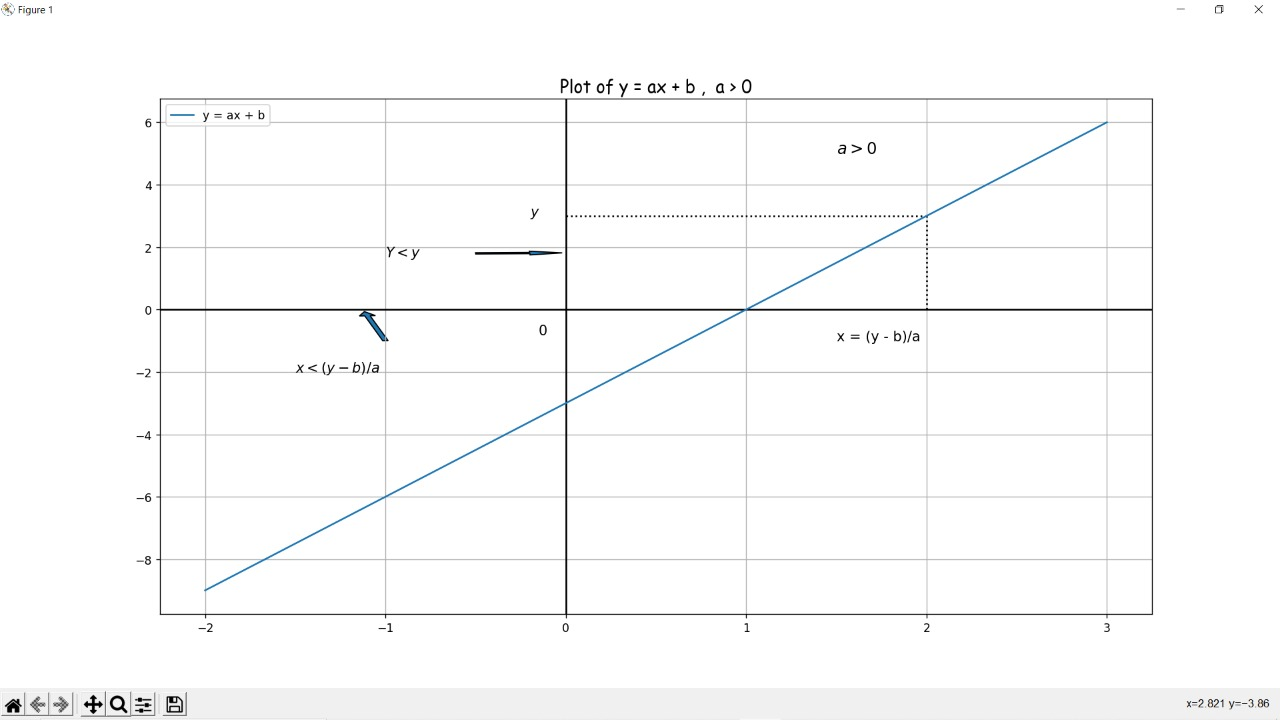
\includegraphics[width=\textwidth,height=6.5cm,keepaspectratio]{figures/Python_code_output.jpeg}
		\caption{FIG 1}
		\label{fig1}
	\end{figure}
\end{frame}

\end{document}
